\documentclass{article}
\usepackage{titling}
\usepackage{scrextend}
\usepackage{xcolor}
\usepackage{graphicx}
\usepackage{tipa}
\usepackage{hyperref}
\usepackage{lipsum}
\usepackage{blindtext}
\usepackage{multicol}
\usepackage[export]{adjustbox}
\usepackage{newspaper}
\usepackage[margin=1in,tmargin=0.75in]{geometry}

\newcommand{\PutTitle}[1]
{
    \begin{center}
        {\huge\bfseries\thetitle}\\
        by \theauthor\\
        \thedate\\
        #1        
    \end{center}
    \hrule
    \vspace{2ex}
}

\setlength\paperwidth{8.5in}
\setlength\paperheight{11in}
\setlength\parindent{24pt}

\hypersetup
{
    colorlinks=true,
    linkcolor=blue,
    urlcolor=blue,
}

\graphicspath{{pics/}}

\title{BINGO Project \#4}
\author{Jonah Mondragon}
\date{\today}

\begin{document}

\PutTitle{English Period 8}
\pagestyle{headings}
\thispagestyle{empty}

\section{Academic Vocabulary Book}
Create a dictionary with the following Academic Vocabulary:
\begin{addmargin}[0.5in]{0in}
    \subsection*{Alliteration}
        A form of rhyme that involves the start of words rather then the end.
    \subsection*{Allusion}
        A subtly implied reference to something external to the context of the implication; often with the purpose of comedic
        effect.
    \subsection*{Characterization}
        The profile of a character; the analysis, or observation, of someone's tendencies or disposition.
    \subsection*{Foreshadowing}
        A reference made within a fictional context referring to a future event; typically a near disaster, or the ending. 
    \subsection*{Homonym}
        Two words with the same sound---with the possibility of sharing the same spelling as well---but with difference in
        meaning.
    \subsection*{Imagery} 
        Language delivered with the purpose of conveying a scene (or an image) to the reader/observer.
    \subsection*{Irony}
        A situation in which an entity's expected behavior is either the exact opposite of reality, or intensely the same.
    \subsection*{Metaphor}
        A methodology used in an either literary or conversational sense to convey a new concept to another person; using 
        their prior knowledge of some other concept; or something simple enough that the connection can be either humorous
        and/or enlightening.
    \subsection*{Monologue}
        An intentional form of rambling; typically put into action when encountered by an immensely dense subject;
        particularly a self-indulged subject.
    \subsection*{Oxymoron}
        A situation where two antonyms are used together to form a practical idea; ``deadly alive''; ``drowned vividness.''
    \subsection*{Persona}
        Only one simple aspect of someone's personality; perhaps as a public figure; or an entity with mannerisms.
    \subsection*{Personification}
        The application of a personality to an otherwise inanimate object; or a more instinctual entity.
    \subsection*{Prologue}
        An introduction; the exact implementation is defined by the application.
    \subsection*{Pun}
        A play on words.
    \subsection*{Rising Action}
        An event, or set of events, that ultimately lead to the climax or the need for the climax.
    \subsection*{Soliloquy}
        The notion whereby one's inner thoughts can converse themselves aloud unconsciously; whether when alone or 
        accompanied by other people. Usually used within observed fictional stories with the intention of allowing the
        audience to understand the concerns/motives of the character.
    \subsection*{Sonnet}
        A poem whose verses contain 14 lines and are generally written via means of iambic pentameter (iambic pentameter
        meaning; 10 syllables on a single line; and one of every two are stressed; a phenomenon that often occurs 
        naturally in the use of English).
    \subsection*{Synonym}
        A word with a similar or interchangeable definition with another; country and county.
    \subsection*{Tableau}
        Imagery with very precise accuracy.
    \subsection*{{\color{red}The{\color{blue}me}}}
        One central idea that many objects involved refer to; in storytelling, it can be thought of as
        ``{\color{red}the}\textpipe{\color{blue}me}ssage.''
\end{addmargin}

\section{Acrostic Poem}
\begin{addmargin}[0.8in]{0.8in}
    Maybe I was too giddy, \\
    Awkward, perhaps; but no; she told me explicitly otherwise. \\
    Reaching around her shoulder; heartrate playing the gypsy; \\
    Inclined to the possibility of stealing a kiss. \\
    Allow my head to tilt toward; or climb inward into a frenzy? \\
    Humbling, hopefully, with the words ``next time''; thus instilling forward bliss. \\
\end{addmargin}

\section{Newspaper}
\vspace{0.5in}
{
\date{February 19, 1598}
\SetPaperName{Verona Times}
\SetPaperPrice{TWO DOLLARS}
\SetPaperSlogan{``I don't remember the books I have read any more then the meals I have eaten; even so, they have made me''}
\SetPaperLocation{Verona, Italy}
\currentvolume{47}
\currentissue{1}
\maketitle

\setlength{\columnsep}{15pt}
\begin{multicols}{3}
    \headline{\sf{The feud of The Montague's and The Capulet's}}
    The only conflict which has plagued our fair city for centuries has been between the Montague's and the Capulet's; two well esteems lineages, with vast influences upon Verona. 
    Chief among these are the Capulet's ownership of Piazza Delle Erbe marketplace; making for an amiable nest egg. 
    On the side of Montague's, they only happen to own the Communal Palace, enough said.
    A recent development has put this age-long feud into a bit of a frenzy.
    Tybalt of the Capulet family, a man whom we haven't much information;\footnote{
        In our attempts to facilitate questions of his stature within the Capulet family, Tybalt managed to evade our every request in a rather amazing fashion; involving showing off several disguises of great dexterity and fashionable uses of his sword.}
        was recently killed by Romeo of the Montague family, surely extenuating the tension of the two families.
    To an utter astonishment, the punishment of this crime was not administered to be death, as is usual for the pretense of murder, but rather banishment;
        this was due to the direct manipulation of the Prince, at who's words resulted in the immediate departure of Romeo, he hasn't been seen since.
    This occurrence can only lead to more brutality on both sides of the spectrum; there's speculation that this wasn't an unprovoked attack, that Tybalt had insinuated the situation; of course speculation also lies in the other direction as well.
    Here at \textit{Verona Times}, we can only hope that future events, such as the Spectacled Burning just a decade ago, doesn't recur as a result of this feud; that it stays within private property, and no innocents are killed.
    \closearticle

    \headline{\bf Revolutionary Dress Apparel}
    Our local clothing store ``Witherfords and Family'' have just created a magnificent new set of apparel, for the (comparatively, within the realm of dress apparel) low, low price of 55 Dollars!
    \begin{center}
    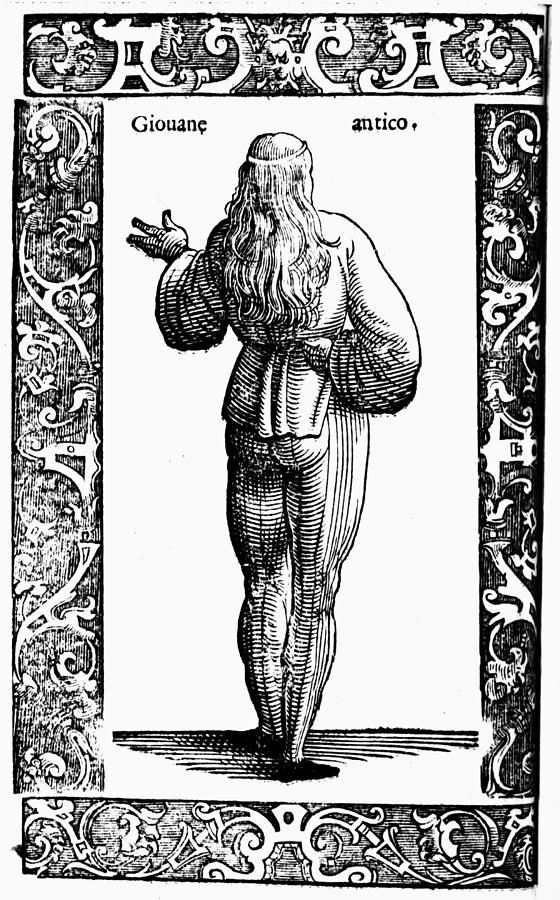
\includegraphics{1598 Fashion.jpeg}
    \end{center}
    \closearticle
    
    \headline{\bfseries Omitted for Brevity...}
    \closearticle
    
    \headline{\ttfamily{Editorial}}
    Long time consumers of the \textit{Verona Times} will know that an editorial section is rarely a concern during it's publication, however it must be emphasized that Romeo is very likely innocent.
    Countless reliable sources tell us so, and the exemption on behalf of the Prince tells significantly of the pretense of this situation; if you happen to see him, on my regard, support him.
    Tybalt was a rather rotten man and not many are supposed to miss him.
    \closearticle
\end{multicols}
}

\section{Artifact Collection}
These are eight artifacts that I believe to be essential to the ideology of Romeo and Juliet; along with a brief explanation of each.
Unfortunately, I was unable to arrange these artifacts into any sort of container, as I couldn't find one large enough to hold a rope ladder and a sword, so hopefully my desktop will suffice.
The paragraph's describing each artifact are present alongside an individual image of them; \#\ref{all_together_now} is an image of all the artifacts together.
I've included my signature in all of the pictures so as to reassure my genuine collection of these artifacts:
\begin{enumerate}
    \item{Letter to Romeo:}\label{letter_to_romeo}
        \begin{center}
            \includegraphics[max width=\textwidth - 6ex]{letter_to_romeo}
            %
\includegraphics[max width=\textwidth - 6ex]{dunce}
        \end{center}
        \paragraph~
        This is the letter that Friar Lawrence was tasked with giving to Romeo; explaining the plan for Romeo and Juliet to escape Verona together.
        Implications of this letter are what make up the tragedy of this story; had this letter succeeded in getting to Romeo, he would have been aware of the plan.
        This aforementioned plan went like this; Juliet would indulge herself with an amalgamated liquid (see artifact \#\ref{vial_of_poison}) made by Friar Lawrence making her appear dead;
            then allowing her an escape from Verona and a reunition with Romeo in Mantua.
    \newpage
    \item{Vial of Poison:}\label{vial_of_poison}
        \begin{center}
            \includegraphics[max width=\textwidth - 6ex]{vial_of_poison}
        \end{center}
        \paragraph~
        Having mentioned the letter to Romeo, at artifact \#\ref{letter_to_romeo}, it becomes pertinent to mention the vial of poison of which the letter-described plan involved.
        This concoction, amalgamated by Friar Lawrence, has the effect of immobilizing its drinker to the point of perceived death, a notion which lasts for forty-eight hours before the drinker then wakes up.
        Use of this concoction was meant for Juliet, with an effort of convincing her family she has died as to enable her to run off with Romeo to Mantua.
        As we later find out, we haven't read up to this point as a class at the time of this writing, this potion is a little too effective and can be attributed to the tragedy of Romeo and Juliet.
    \item{Romeo's Sword:}\label{sword}
        \begin{center}
            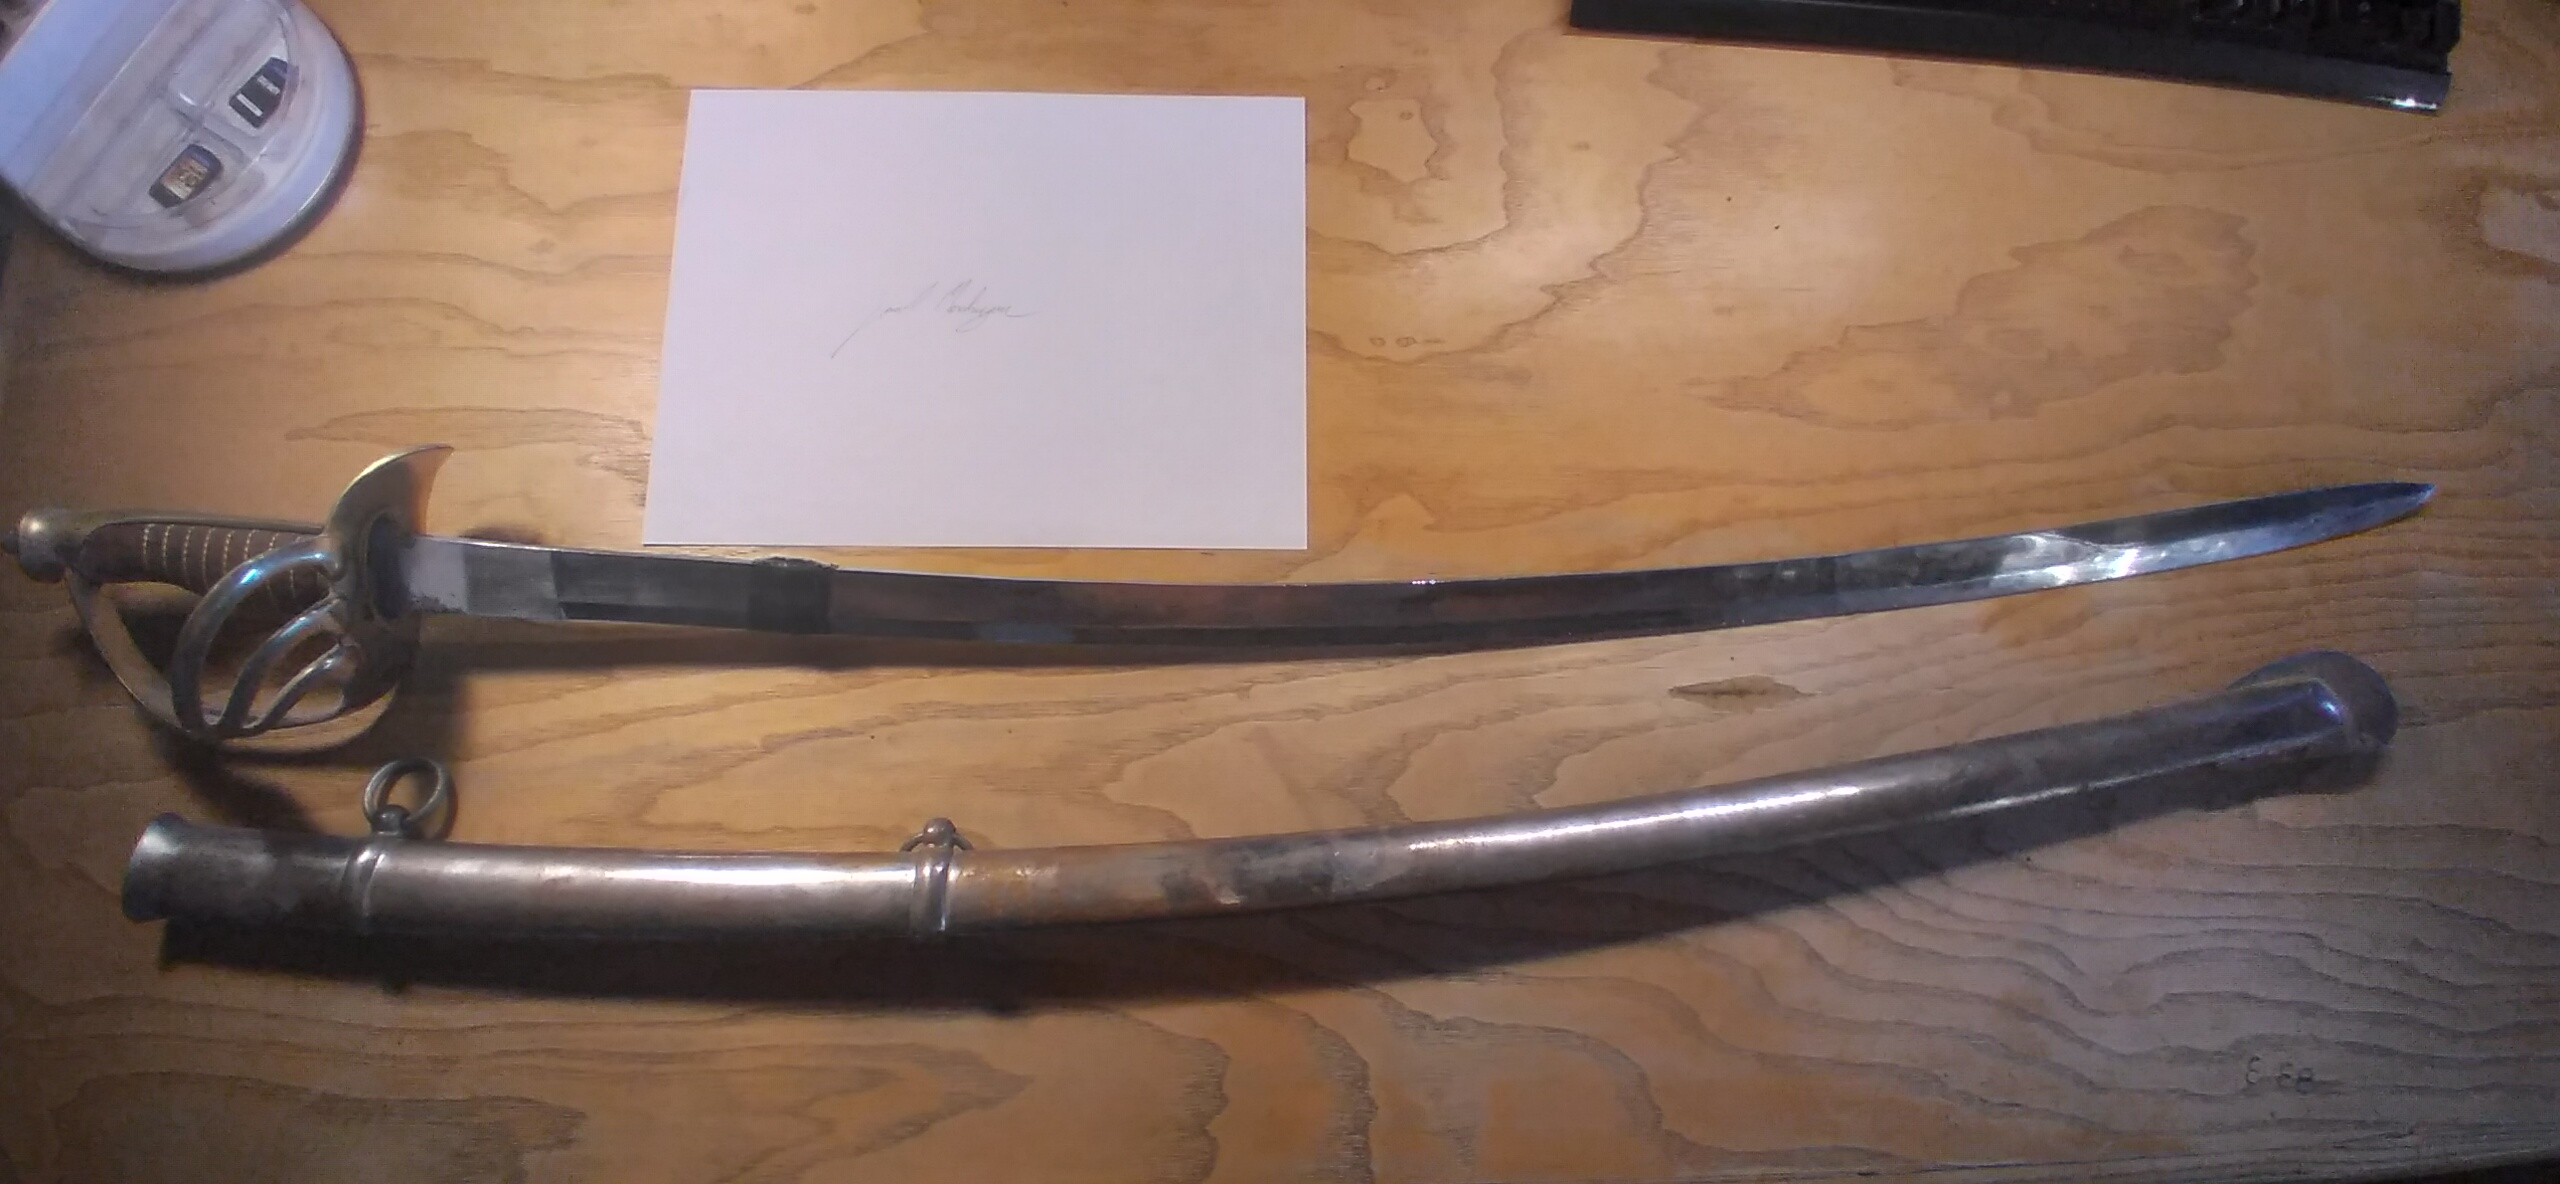
\includegraphics[max width=\textwidth - 6ex]{sword}
        \end{center}
        \paragraph~
        Use of swords is a major writing point in Romeo and Juliet owing to the time of it's inscription; sword-play was the primary device of any altercation throughout.
        Two examples of these manipulations, of swords as devices; \textit{Act I Scene I} in which the Montague and Capulet feud is introduced through the drawing of several swords during an altercation;
            \textit{Act III Scene I} which is the fight between Tybalt and Romeo; the latter being pertinent to my choice of this item.
        The fight between Tybalt and Romeo is pivotal to the plot, the upshot is Romeo becomes ``banishèd,'' archaic spelling I'm sure, after killing Tybalt with a sword;
            without the presence of this altercation, there would be no need for Romeo and Juliet to flee from Verona; no mix-up with the vial of poison.
        The sword in the image above represents the one Romeo wielded throughout the play.
    \item{Romeo's Dagger:}
        \begin{center}
            \includegraphics[max width=\textwidth - 6ex]{dagger}
        \end{center}
        \paragraph~
        Seeing as \#\ref{sword} presents Romeo's sword, it seems only natural to present his dagger immediately afterward.
        This is the dagger Juliet keeps with her in bed during \textit{Act IV}, and ultimately kills herself with in \textit{Act V}.
        As well as with swords, daggers are used as an altercation alleviation device throughout Romeo and Juliet.
        While only a few characters (Romeo, Juliet, Lord Capulet, Peter, and two extra musicians) ever interact with a dagger, whether verbally or 
            physically, it's purpose is definite because of it's use regarding Juliet.
    \item{Rope Ladder:}
        \begin{center}
            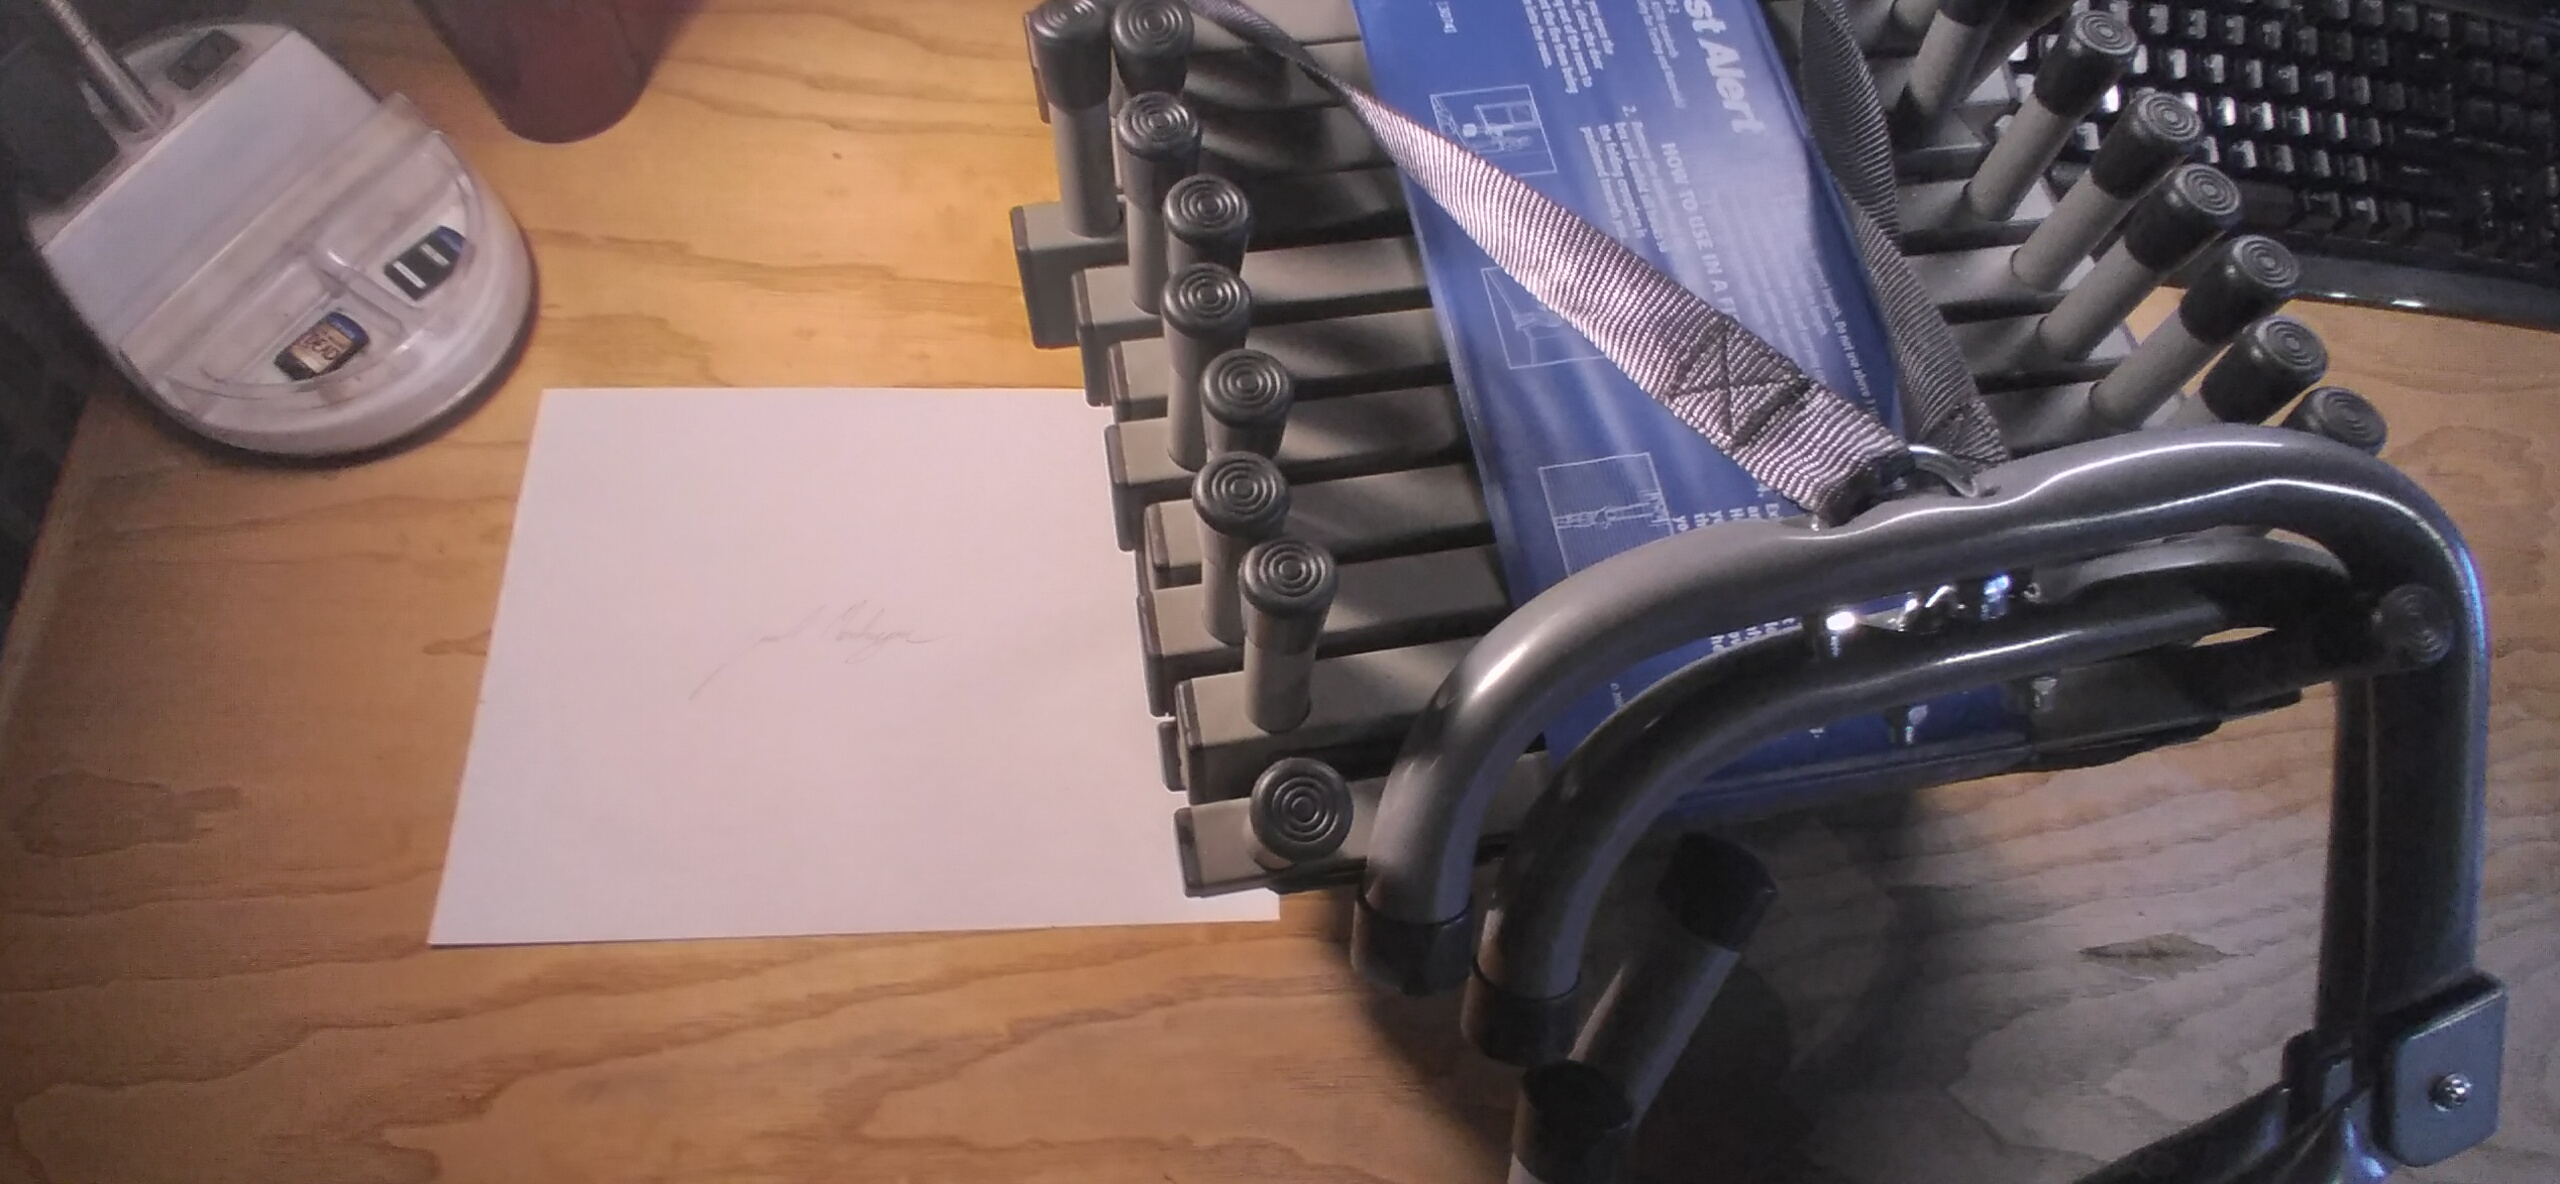
\includegraphics[max width=\textwidth - 6ex]{rope_ladder}
        \end{center}
        \paragraph~
        A rope ladder makes an appearance in \textit{Act III Scene III} during an exchange involving Juliet and the Nurse; Nurse was bringing it for Romeo's use as an entrance device for Romeo and Juliet's wedding night.
        The pertinence of a rope ladder to the plot is, while weak, relatively simple; it represents the means by which the supposed wedding would initiate had the fight between Tybalt and Romeo not occurred (see artifact \#\ref{sword}).
        The rope ladder in the image above is meant to represent the same one that was to be used by Romeo during \textit{Act III Scene III}.
    \newpage
    \item{Herbs and Flowers:}
        \begin{center}
            \includegraphics[max width=\textwidth - 6ex]{herbs_and_flowers}
        \end{center}
        \paragraph~
        Herbs and flowers make their only appearance in \textit{Act II Scene III} in a metaphor for human behavior.
        In this aforementioned scene, Friar Lawrence describes both ``man as well as herbs'' as being ``naught so vile'' as well as ``Nor aught so good,'' describing the struggle of good and evil with humans; the metaphor relating to the properties of 
            herbs and flowers as being either poisonous or liberating.
        This metaphor has pertinence to the plot, again an admittedly weak pertinence, because of the Montague and Capulet feud; which is good and which is evil?
        Naught can tell.
    \item{Juliet's Ring:}
        \begin{center}
            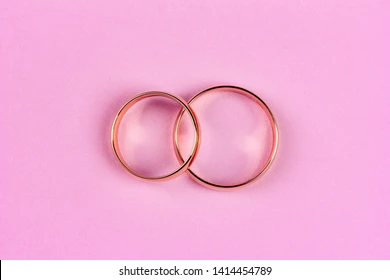
\includegraphics[max width=\textwidth - 6ex]{ring}
            %
\includegraphics[max width=\textwidth - 6ex]{dunce}
        \end{center}
        \paragraph~
        The ring depicted above is meant to be Juliet's ring (which first appears in \textit{Act III Scene III}).
        This ring was to be given to Romeo by way of the Nurse after the death of Tybalt; meant as a remembrance of their love.
        After Juliet's death, Romeo takes her ring from her body, a final act of nihilism regarding her life.
    \newpage
    \item{Juliet's Necklace:}
        \begin{center}
            \includegraphics[max width=\textwidth - 6ex]{necklace}
        \end{center}
        \paragraph~
        My reason for this choice is rather dense; it boils down to religious imagery; a necklace also isn't ever directly referenced in the play, but is referenced in the movie 
        ({\color{blue}\underline{\href{https://www.boxofficemojo.com/release/rl2305590785/weekend/}{Romeo + Juliet}}}).
        The actual necklace used in the movie has a cross attached to it, I could not procure a necklace of this nature, relating to the religious imagery presented throughout.
        A few of these religious references are predominately present in the original marriage scene (\textit{Act II Scene V}); details of which are too verbose to be detailed.
    \item{{\color{blue}\underline{\href{https://www.youtube.com/watch?v=73lj5qJbrms}{All Together Now}}}:}\label{all_together_now}
        \begin{center}
            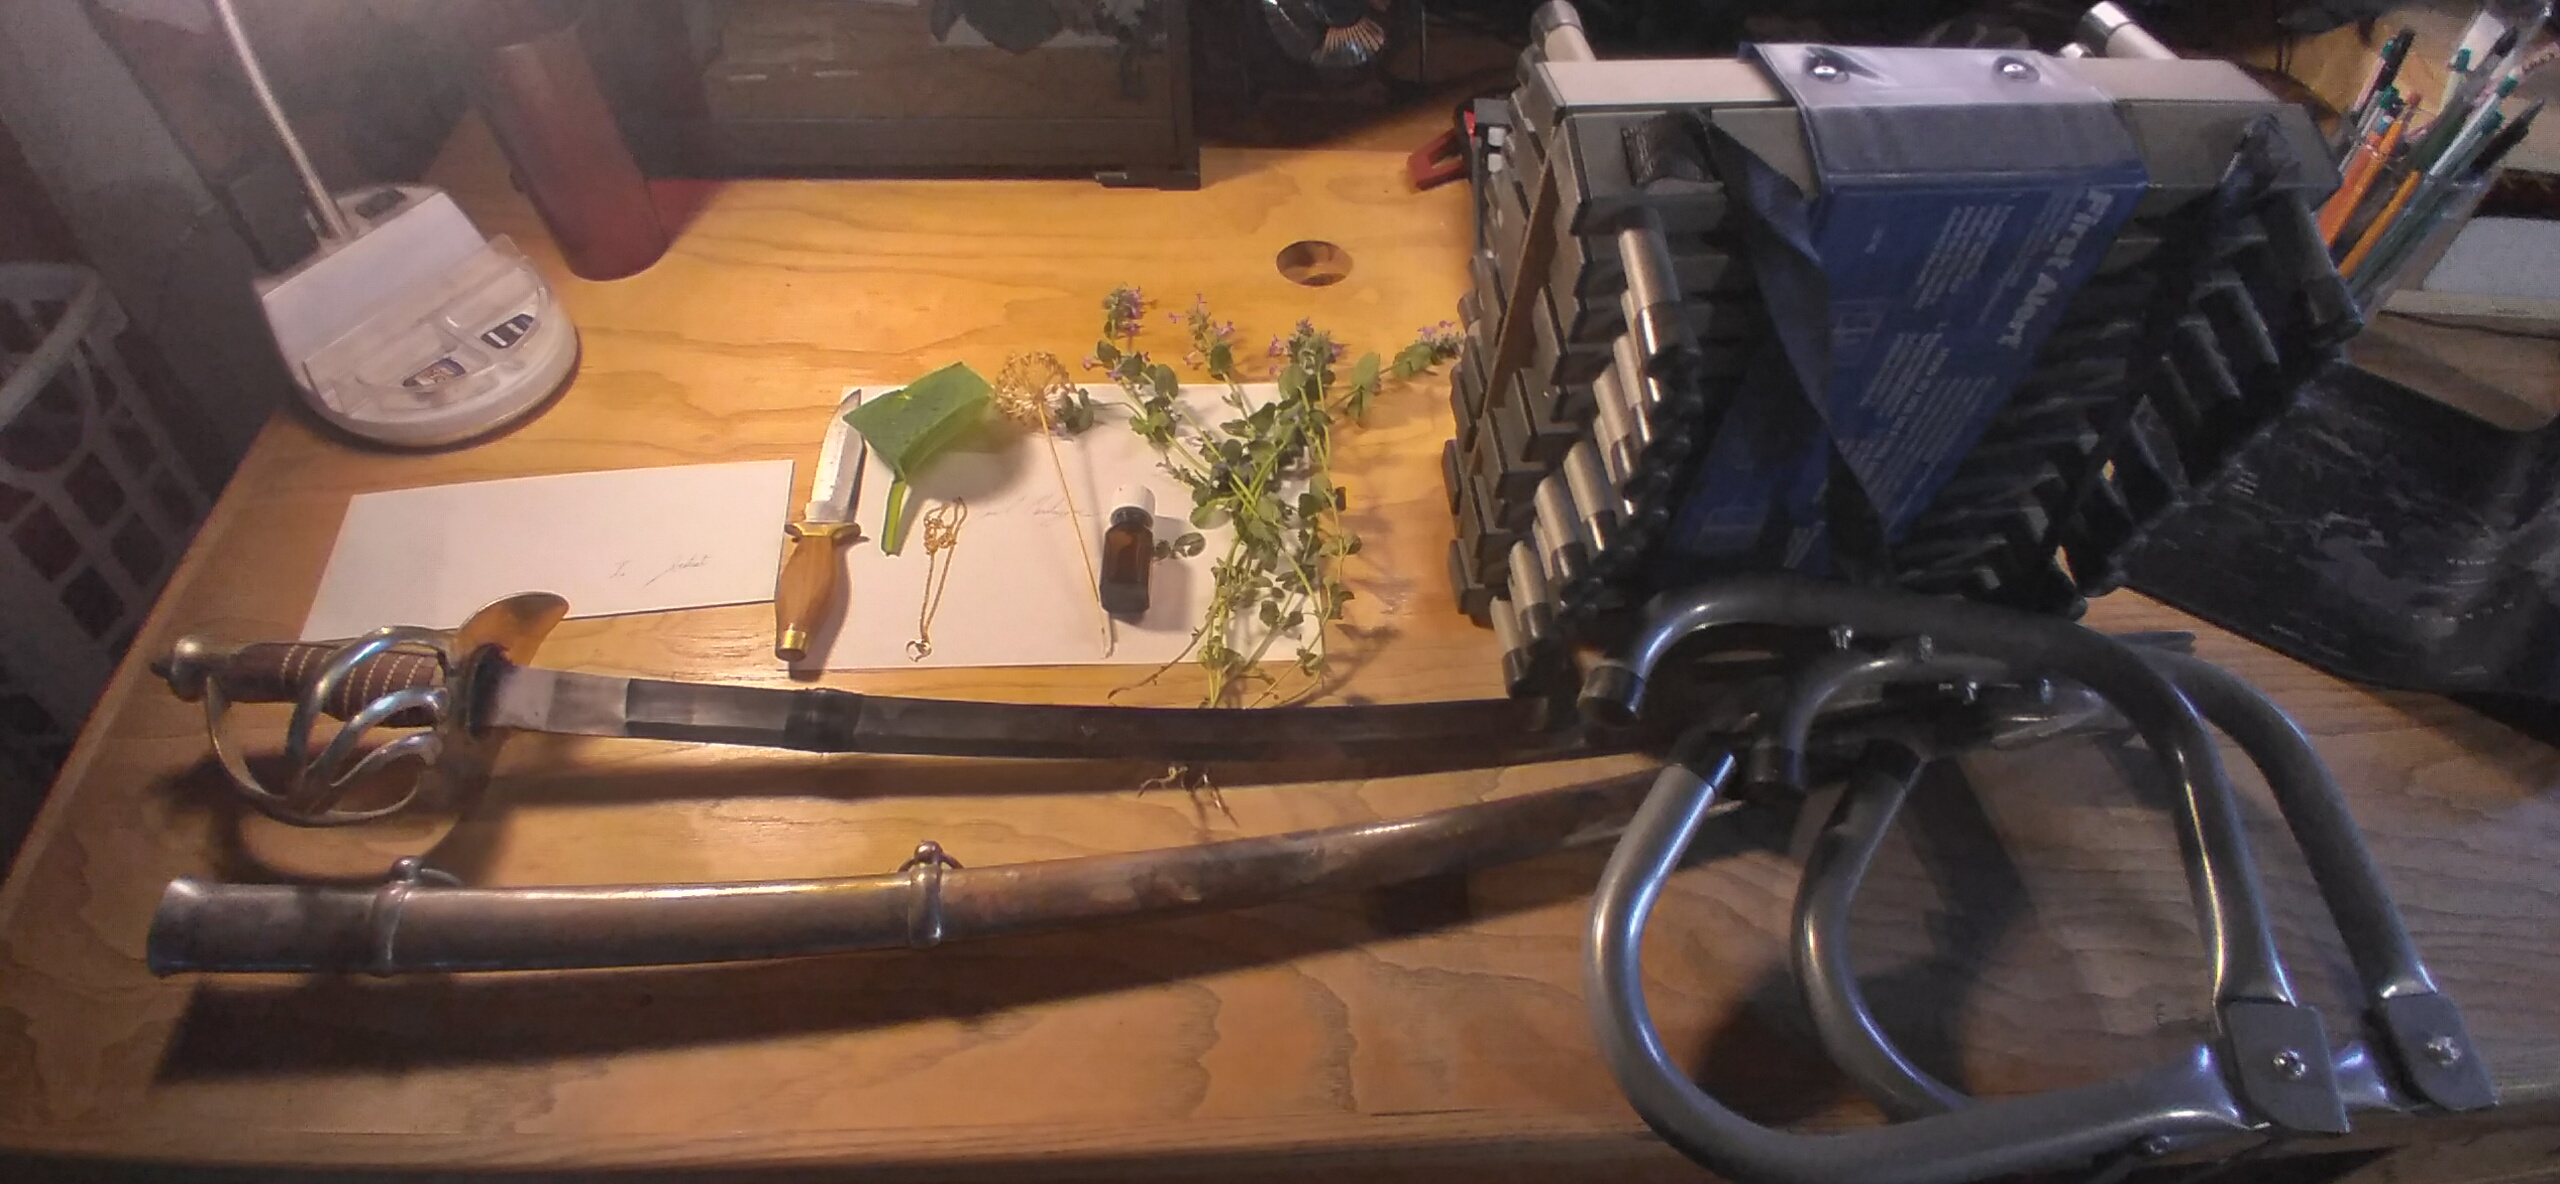
\includegraphics[max width=\textwidth - 6ex]{all_together_now}
            %
\includegraphics[max width=\textwidth - 6ex]{dunce}
        \end{center}
\end{enumerate}

%\section{Original Movie Poster}

\end{document}
